To evaluate the produced \ac{ECD} topologies, topologies are represented as a hypergraph, therefore the basic theory of hypergraphs first should be explained.
Hypergraphs are a generalization of a graph and are formally defined as:
$H = (V, E)$, where $V$ is a set of $N \in \N$ vertices $\{v_1,...,v_N\}$ and $E$ is a set of $M \in \N$ hyperedges $\{e_1,...,e_M\}$, where each hyperedge $e_i \in E$ is $e_i \subseteq V$. \cite{hypergraph_def}
In matrix notation a hypergraph can be represented in a so called adjacency matrix.
An example of an adjacency matrix together with the corresponding drawing of a hypergraph can be found in figure \ref{fig:hypergraph_adjacency}.

\begin{figure}
\begin{center}
    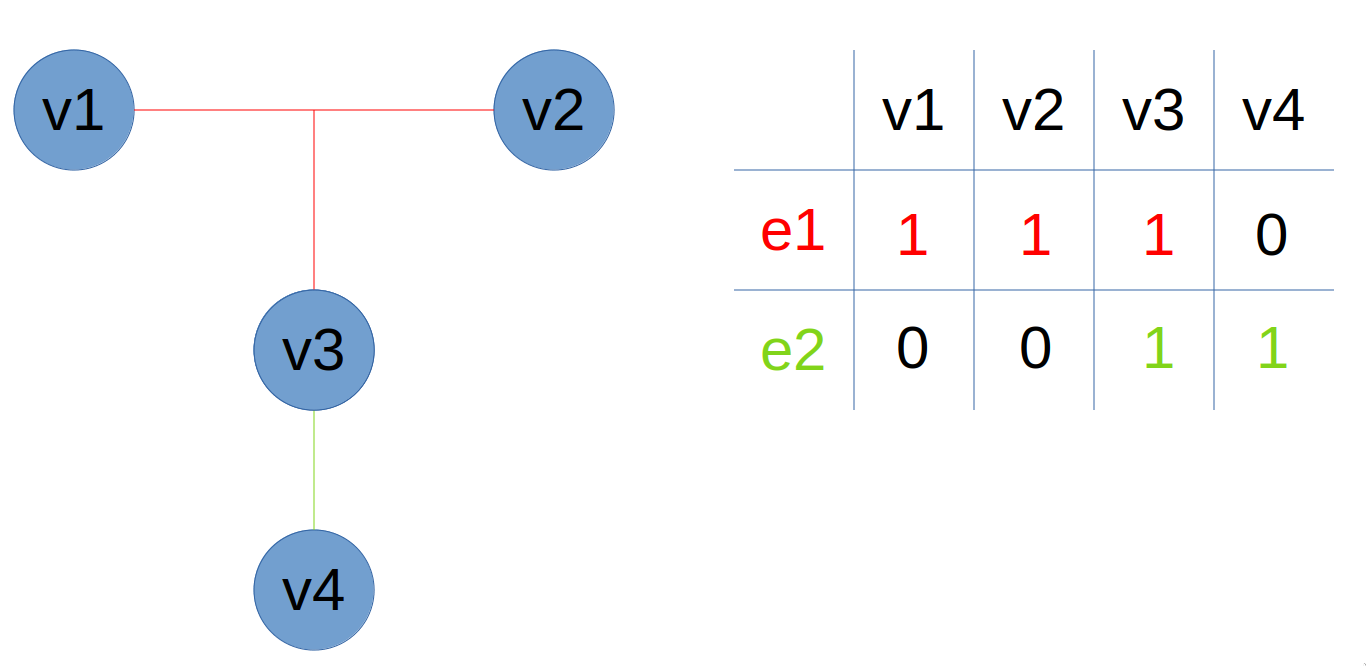
\includegraphics[width=13cm]{imgs/hypergraph_adjacency.png}
    \caption{An example drawing of a hypergraph with its corresponding adjacency matrix. The hypergraph is defined as: $H = (V, E)$, $V = \{v1, v2, v3, v4\}$, $E = \{e1, e2\}$, with $e1 = \{v1, v2, v3\}$, $e2 = \{v3, v4\}$. In the adjacency matrix a row corresponds to a hyperedge and each column to a vertex. When a vertex is present in a hyperedge it has a 1 as an entry in the matrix, when a vertex is not present it has a 0.}
    \label{fig:hypergraph_adjacency}
\end{center}
\end{figure}
